\chapter{Characterizing Adhesion in Multiple Myeloma Cells}
\label{Chap:Adhesion}

\section{Introduction}The ability of a cell to mechanically interact with its environment is critically important to almost all aspects of cell biology and plays critical roles in many processes from development to immune response \cite{Halbleib2006,Springer1990,Springer1987}. These mechanical interactions between cells and their environment are mediated by adhesion molecules present on a cell's surface which enable the cell to physically attach to surrounding cells and structural molecules present in the environment \cite{Hay2013, Gumbiner1996}. Cell adhesion mediates a cascade downstream effects which can result in significant changes in cell function and behavior \cite{Schlie-Wolter2013}. Many cell types require adhesion to other cells or structural molecules for survival and a lack of adhesion or lack of the appropriate extracellular matrix (ECM) components can result in a specific form of apoptosis known as anoikis \cite{Gilmore2005}. Anoikis prevents cells growing in contextually inappropriate locations and is important for maintaining the integrity of tissues in the body \cite{Gilmore2005}. In cancer, resistance to anoikis removes a tumor cell's dependence on adherence for survival, is considered a hallmark of cancer and is believed to be a requirement for cell survival in the bloodstream leading to metastasis \cite{Paoli20133481}. Multiple myeloma (MM) is a hematopoietic malignancy where the enhanced adhesion characteristics to ECM components and other cells in the bone marrow microenvironment mark increasing capacity for the cancer to interact with its microenvironment advancing tumor progression, immune evasion, and drug resistance \cite{Chauhan1996, Damiano2000, Gorgun2013, Jourdan1998b, Shain2001}. Characterizing adhesion in multiple myeloma can lead to an understanding of how tumor cells acquire to specific molecules, changes that occur once cells are adhered, and how drug resistance is acquired because of adherent populations of MM cells.

There are several techniques used to characterize adhesion but they all have tradeoffs which limit their impact. Macroscale adhesion assays are well suited for characterizing adhesion properties of populations of cells. A typical macroscale adhesion assay involves functionalizing the surface of a well-plate with an ECM protein or cell-bound molecule, or even cell population and allowing the seeded cells to settle to the bottom where they may adhere to the surface. After an incubation time, cells are washed with a micropipette, non-adherent cells are washed away while adherent cells remain at the surface of the well-plate. This approach results in the fractionation of cells into two populations based on their adherence characteristics. The adherent and non-adherent populations can be separated and interrogated following the assay with biochemical characterization methods .

Beyond this technique there are several microscale approaches to characterizing adhesion in populations of cells. Unlike their macroscale counterparts, microscale adhesion assays offer the potential to collect quantitative data about shear stresses required to dislodge cells and provide single-cell resolution. Microscale adhesion assays typically involve functionalizing a microchannel with a protein, molecule, or cell type of interest and observing the channel using microscopy. Detachment assays setup like their macroscale counterparts, first allowing cells to settle onto the surface then by observing individual cell detachment from the surface with increasing flow rates. Microscale attachment assays flow cells into functionalized microchannels and modulating the flow rate from high to low, observing the flow at which individual cells adhere to the surface \cite{Yang2013, Lamorte2012}.

Macroscale adhesion assays are best suited for populations of cells with binary adhesion characteristics. Since these assays require pipetting which ideally operate at a single shear rate (though there are many factors that will affect shear) cells are separated into only two subpopulations, subtleties within a heterogeneous population will be largely unobservable. The largest benefit of macroscale adhesion assays is their ease of use and the ability to retain or collect cells from both adherent and non-adherent populations for further characterization. Microscale assays perform well characterizing single cells and can elucidate subtleties and transitions within complex populations. Unfortunately, the microchannel design requires flow through a channel. The flow through means that cells that are not adherent over the course of the assay will be washed away into the waste and post-assay characterization of individual cells is challenging \cite{C2IB20036H, Andersson2003, ELPS200305627}. 

In spite of cell-based microscale devices being touted for their ability to minimize reagent use, due to their design, microchannel-based adhesion assays end up losing many cells to waste. The large amount of cell waste prevents these highly quantitative platforms from being utilized to analyze small-sized samples such as those isolated from patients. Warrick \textit{et al.} was capable of developing a quantitative microscale adhesion analysis by using using controllable oscillatory flow within a microchannel, preventing cells from being washed away. \cite{Warrick2013}. This platform enables adhesion assays with limited samples but does not address the need to further characterize cells once their adhesion characteristics have been determined. We present an adhesion assay that utilizes the oscillatory flow technique developed by Warrick \textit{et al.} and adds further functionality by implementing technique using photocrosslinkable gel to "freeze" cells \textit{in situ} immediately following the adhesion assay, allowing enhanced interrogation of each cell. We apply and validate this technique to cell lines and to cells isolated from multiple myeloma patients to better understand how adhesion plays a role in MM disease progression and drug resistance. 

\section{Methods}

\subsection{Device fabrication and preparation}
Adhesion devices were fabricated according to the protocol used by Warrick \textit{et al.} \cite{Warrick2013} using polydimethylsiloxane for the channel layer and device membrane and slide glass for the floor of the device. Device assembly was achieved using two-sided tape that was pattered via xerography using a plotter cutter.

Devices were functionalized with three different surface treatments with molecules multiple myeloma cells have been reported adhering to in the bone marrow microenvironment. These surface treatments are VCAM, ICAM, and hyaluronic acid (HA). The devices were treated as follows: Device components were oxygen plasma treated at 50W for 30 seconds. Devices were then assembled on the benchtop then exposed to germicidal UV light for 20 minutes. In sterile conditions, devices were filled with 100 \textmu g/mL either VCAM, ICAM, or HA in 1X PBS. A control condition was filled with 1X PBS. Filled devices were placed in an incubator for 2 hours. Following incubation, devices were flushed with 1X PBS for at least three volume replacements then returned to the incubator for at least 1 hour before use.

In experiments using patient cells, CD138+ cells were isolated from patient bone marrow aspirates as described previously \cite{Pak2015}. Cell line experiments used the MM lines RPMI8226 and MM.1S. Prior to the adhesion assay being run RPMI8226 cells were stained with Hoechst and MM.1S cells were stained with cell tracker red. 

Crosslinkable media was prepared using the PEG-diacrylate and lithium phenyl-2,4,6-trimethylbenzoylphosphinate photocrosslinkable protocol as described by Fairbanks \textit{et al. } \cite{Fairbanks2009}. Cells were added to the media at 200 cells/\textmu L.

Devices were prepared for operation by first thoroughly washing the channels out with crosslinking media. 10 \textmu L of media was removed and replaced with 10 \textmu L of cell suspension. The device membrane is carefully placed on the outlet of the device and is tapped several times to ensure that a seal has been made and to distribute cells from the port into the channel. The loaded device is taken to the microscope where the assay is performed. 


\subsection{Platform operation}
The cell-loaded device was placed on the microscope and the tip of the piezo actuator is placed to barely touch the top of the membrane. The assay is performed by initiating programmed oscillation the piezo actuator and simultaneously beginning image acquisition. The oscillatory program sweeps in a sawtooth waveform from 1 Hz to 0.1 Hz over the course of 5 minutes. Higher oscillation frequencies result in higher flow and shear within the channel. 

Following completion of the adhesion component of the assay, the field of view of the channel that was observed for the adhesion assay is exposed to UV light from the microscope's DAPI filter initiating crosslinking of the PEG in the channel fixing the cells in place allowing for further downstream analysis. 

The device is disassembled by removing the PDMS lid from the glass bottom then the cells within the gel are fixed. The fixed cells can be further analyzed and characterized. We stained MM.1S and RPMI cell lines with CD11a and CD227 within the channel.The stained cells were imaged at high magnification. 


\subsection{Adhesion analysis}

Images captured during the assay were processed using J'experiment (JEX) an image processing suite that utilizes the ImageJ framework \cite{Warrick2016, Warrick2013}. Image sets were reduced in size to conserve memory and hard drive space. Images were processed to identify cells in each framed captured. Cells were saved as regions of interest (ROIs) with their x and y positions within the frame recorded and saved within text files. Text files containing ROI the ROI data were uploaded to the University of Wisconsin HTCondor high throughput computer cluster for processing. Cells or ROIs were tracked between frames using a custom developed particle tracking package for R. The particle tracking package enabled cells to be tracked throughout the course of the experiment from high to low flow rates and enabled the cell's velocity to be determined. Cells with a low enough velocity were considered adhered while those above the threshold velocity were not adhered. The analyzed ROI files were collected form HTCondor where the analyzed data could be reviewed. 

Stained cells from the assay were imaged and registered to the final time point of the adhesion assay with a user-guided registration algorithm developed in-house. 

\section{Results \& discussion}

The adhesion assay presented is modeled on the one developed by Warrick \textit{et al.} though it brings several improvements. The first being increased control over the shear experienced by the cells in the channel. The piezo actuator is driven by a 32-bit Arudino Due (Figure \ref{figure:AdFig1}A) which executes a programmed, repeatable, and robust cycle of high to low shear stresses. Previously frequency of oscillation was controlled manually by a standard laboratory frequency generator. This automation aspect enables raw data to be fed into analysis algorithms with minimal user input streamlining data processing. This assay also results in a large quantity of images being created for each channel run. The addition of frequency automation enables downsampling of the images acquired from approximately 8000 to 2000 images resulting in significant reduction of data set size without loss of adhesion information.

The device design (Figure \ref{figure:AdFig2}B) remains relatively unchanged from the previous version with the exception of the assembly method. The channel itself is now composed of a medical grade two-sided tape which has minimal height variation which is important to maintaining a constant shear between replicates. Additionally the two-sided tape reverse ably bonds the PDMS "lid" of the device to the glass bottom. Being able to remove the lid of the device allows direct access to the culture after bonding avoiding diffusion limitation issues that would prevent reasonable immunocytochemistry staining times. 


\begin{figure}[ht] %DONE
\centering
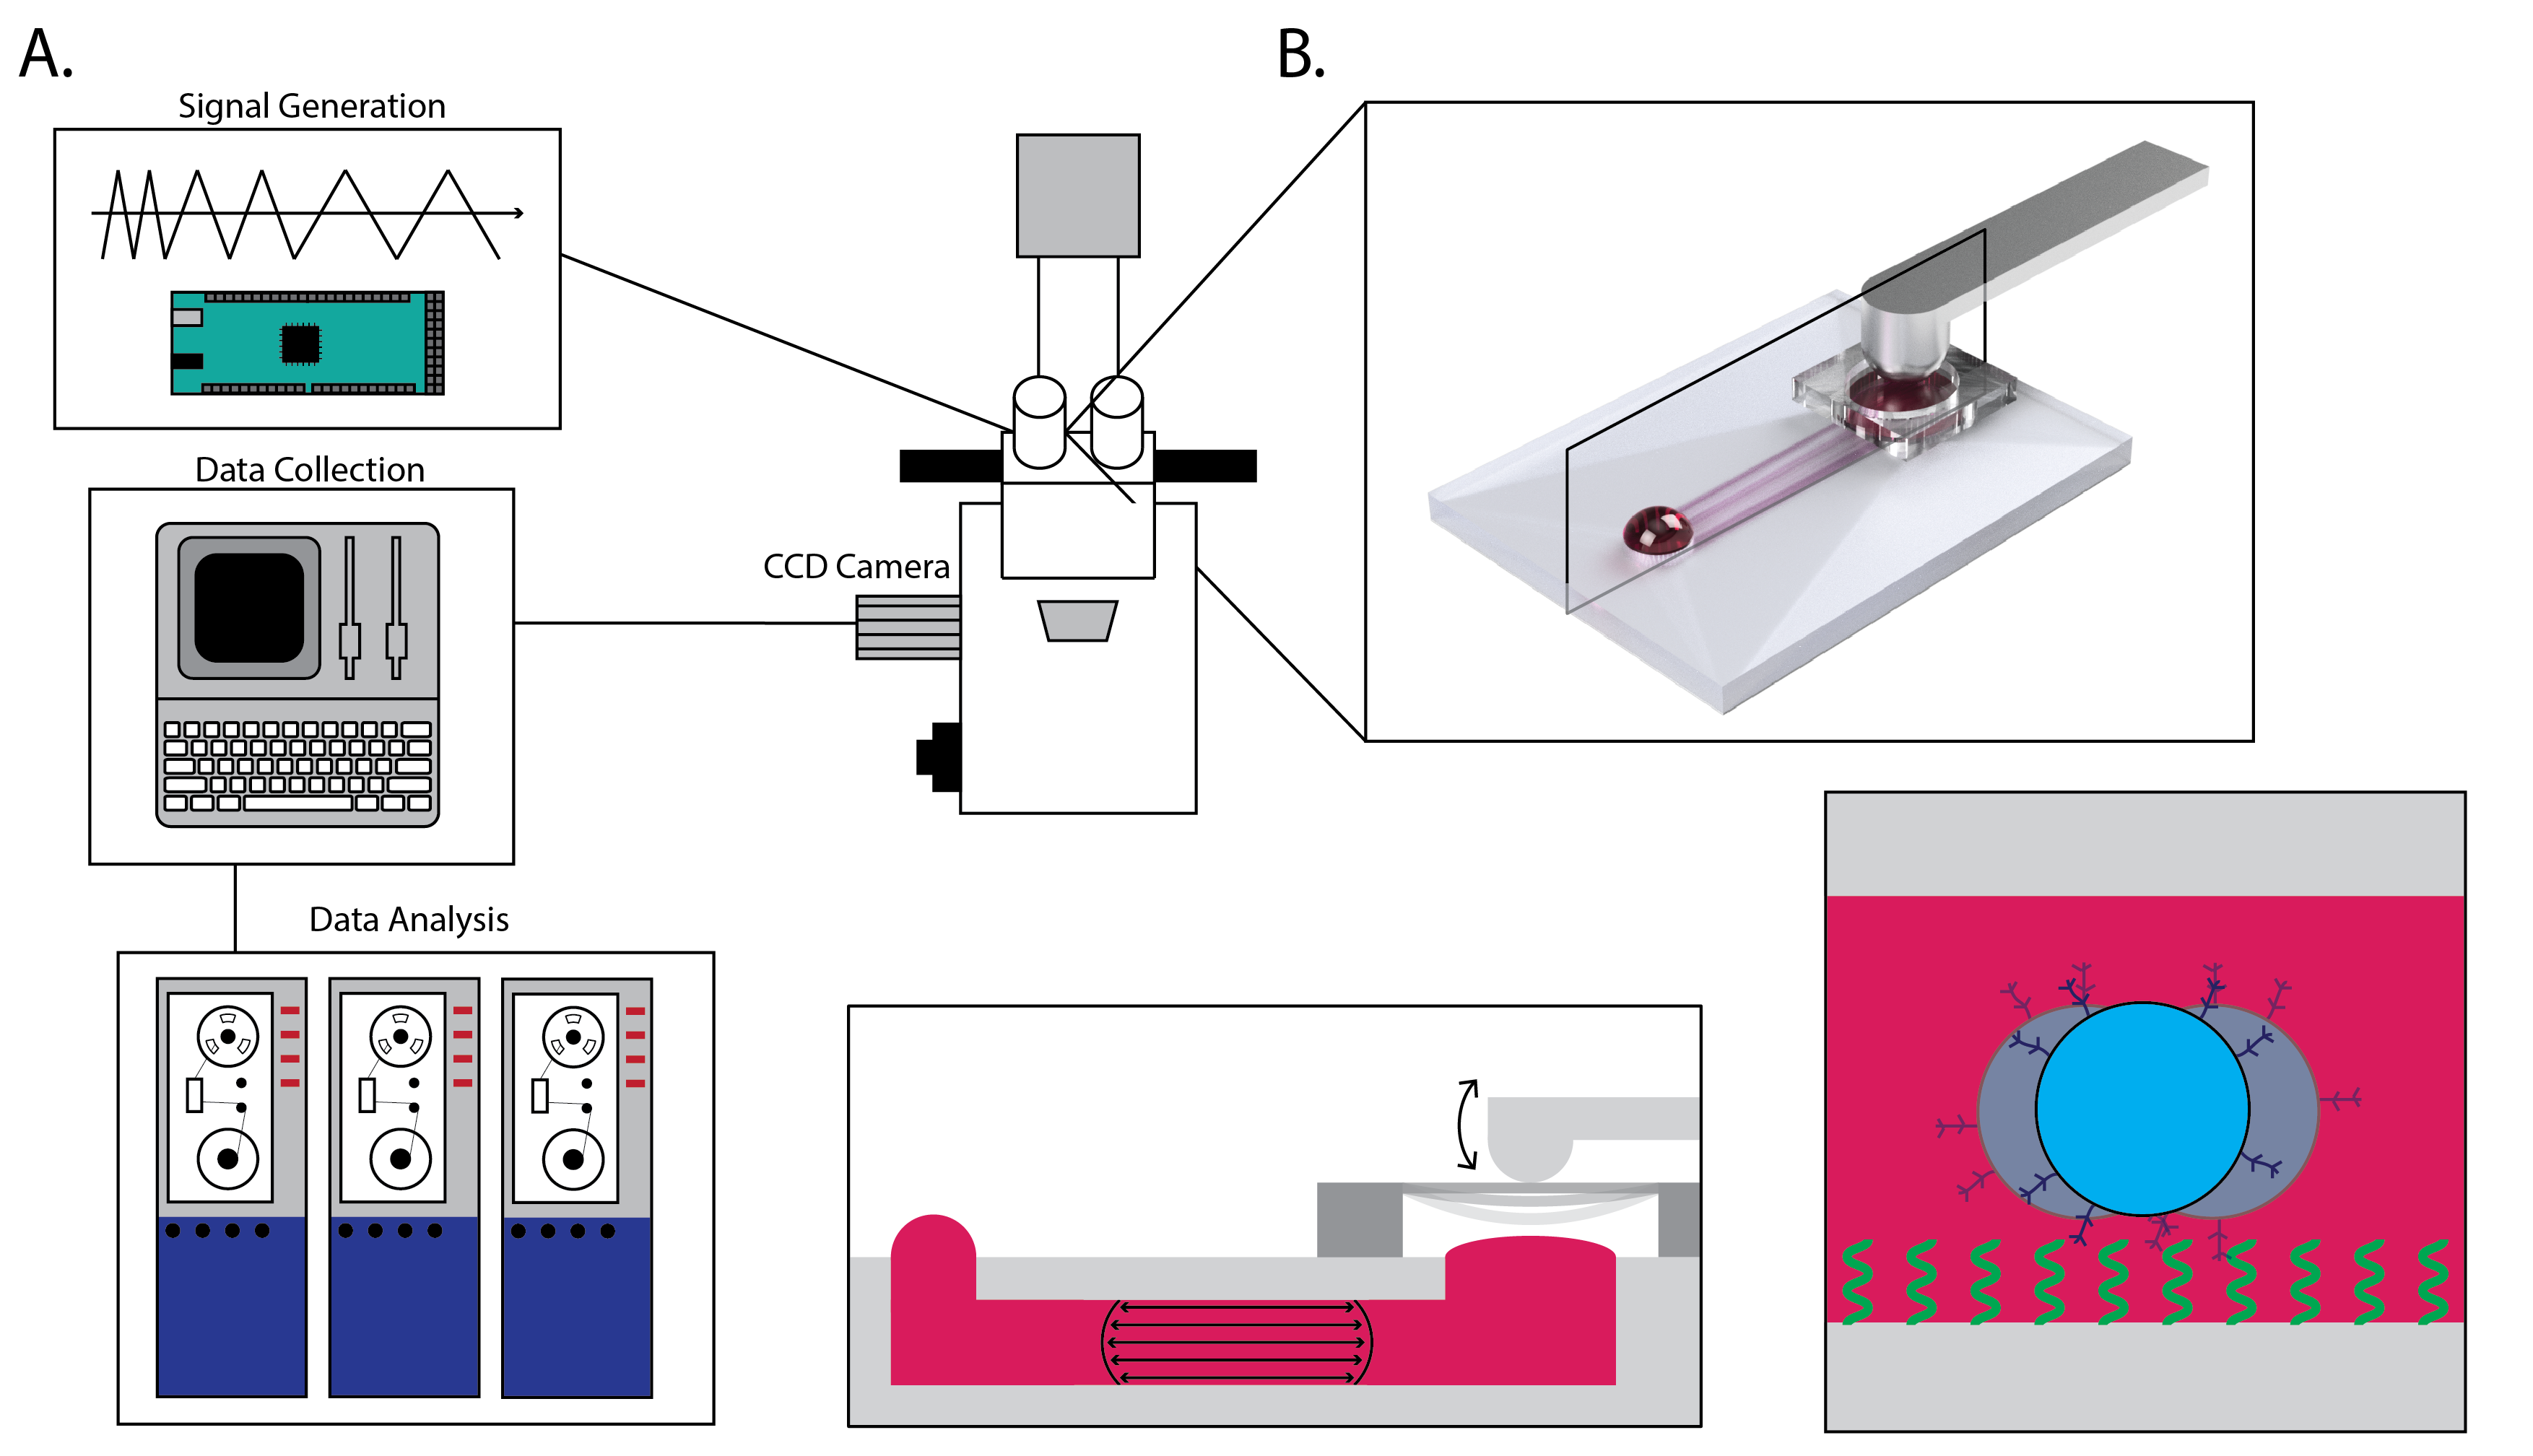
\includegraphics[width=5.75in]{/AdFig1.png}
\caption[\textbf{Adhesion assay schema}]{\textbf{Adhesion assay schema} A) Electronic components of adhesion assay. From top to bottom: Signal generator for piezo actuator, image collection from microscope-attached computer, data analysis performed by HTCondor. B) Adhesion device in increasing detail. From top to bottom: Complete adhesion channel with PDMS membrane and piezo actuator engaged, cross section of adhesion channel showing motion of actuator and fluid within the channel, representation of cell in channel oscillating on the surface of a functionalized channel.}
\label{figure:AdFig1}
\end{figure}

Prior to implementing the photocrosslinking protocol we were able to analyze several MM patient samples with the adhesion assay with three relevant adhesion molecules found in the bone marrow microenvironemnt: VCAM, ICAM-1, and HA \cite{Hideshima2001, Damiano2000, Vincent2005, Reagan2012, Balakumaran2010, Ohwada2008, Vincent2005}. We determined an average frequency of adhesion for each patient on each of the surfaces used (Figure \ref{figure:AdFig2}). To mitigate effects resulting from sample age, the order in which surfaces were tested was performed at random. The order in which the data is presented in Figure \ref{figure:AdFig2} was according to sample behavior with the first three samples having markedly higher mean adhesion frequency in the control condition as well as the VCAM condition and little adhesion in ICAM and HA conditions. VCAM is expressed on bone marrow stromal cells which binding of MM cells has shown to contribute to drug resistance \cite{


\begin{figure}[ht] %DONE
\centering
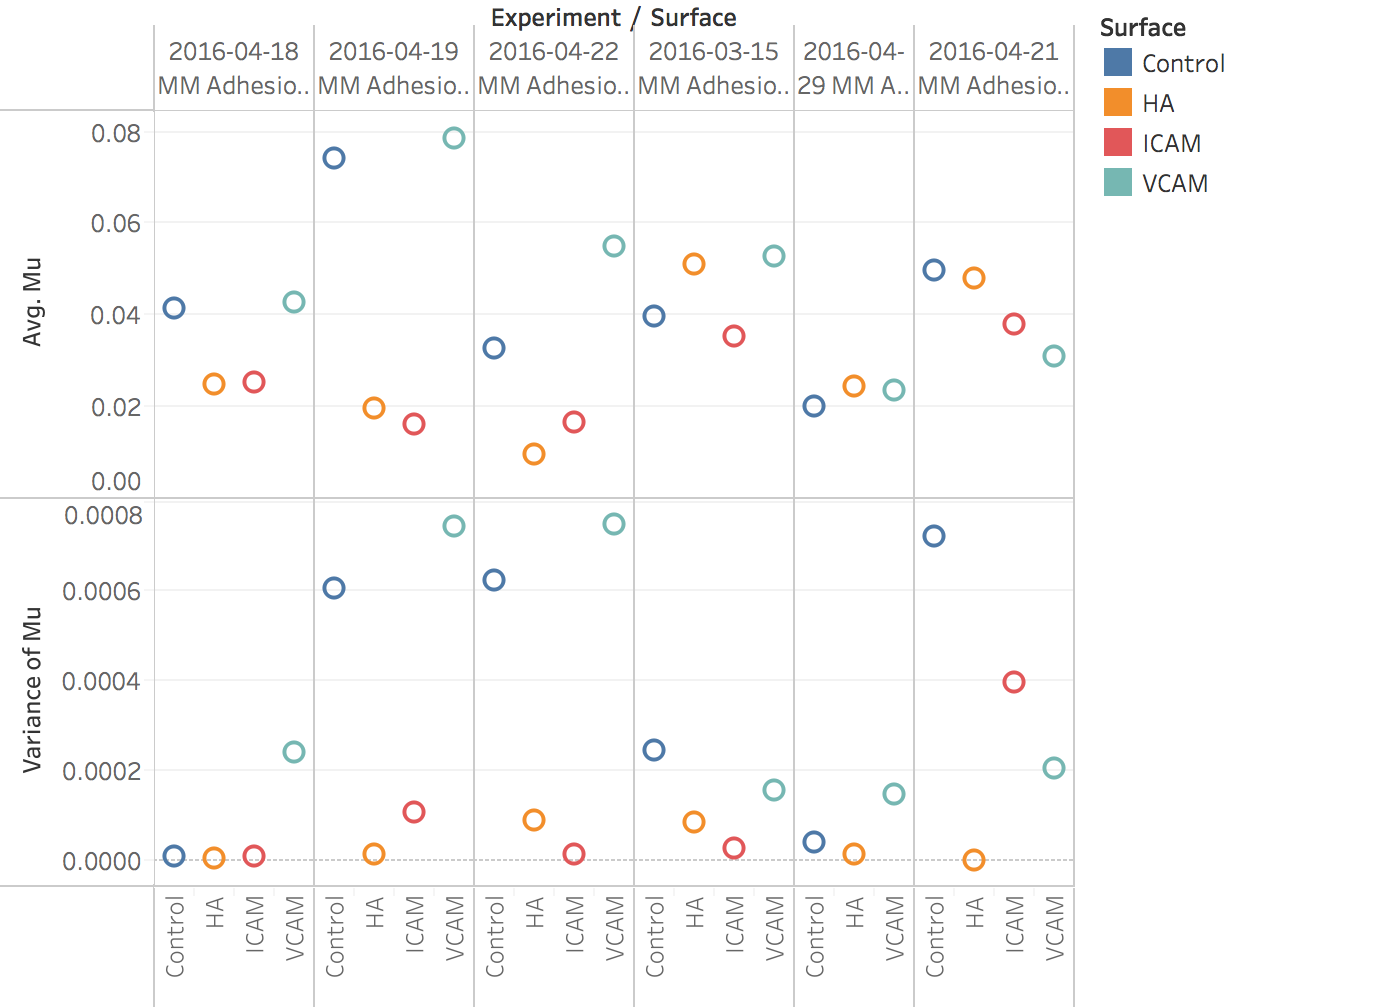
\includegraphics[width=5.75in]{/AdFig2.png}
\caption[\textbf{Aggregate patient adhesion data}]{\textbf{Aggregate patient adhesion data} Top: Frequency of oscillation at which average cell adheres to surface of channel bottom. Bottom: Variance of mean adhesion frequency for each condition and patient.}
\label{figure:AdFig2}
\end{figure}

\section{Conclusions \& future works}